\documentclass{article}
\usepackage[utf8]{inputenc}

\title{Survey on Discrete Wavelet Transforms Using GPU}
\author{Samuel Li}
\date{April 2015}

%\usepackage{natbib}
\usepackage{graphicx}
\usepackage{color}
\newcommand{\fix}[1]{\textcolor{red}{#1}} %Put words in Red

\begin{document}

\maketitle

\begin{abstract}
Discrete Wavelet Transform (DWT) is widely used in data reduction applications.
%
However, such transforms are relatively computationally intensive.
%
To accelerate the calculation of DWT, researchers have applied various parallel
computing techniques, based on the distributed memory architecture~\cite{
chadha2002scalable, woo1995parallel, uhl1996wavelet, nielsen1997scalable}
and the shared memory architecture~\cite{
lucka2000parallel, uhl2000optimization,kutil1999hardware}.
%
In the recent years, the many-core architecture, such as GPU acceleration 
cards, have emerged in the parallel computing field.
%
In this survey paper, we cover many topics regarding calculation of DWT on GPUs.
%
More specifically, we start the survey from technical discussion and evaluation
of implementing the DWT on GPUs~\cite{tenllado2008parallel, van2011accelerating,
garcia2005gpu}.
%
Then we present a few successful use cases of GPU in parallel DWT~\cite{
strengert2004hierarchical, strengert2006pyramid, wong2007discrete,
treib2012turbulence}.
%
Finally, to prepare for the exascale computing, we survey the use of 
heterogeneous architecture with GPUs and multi-core CPUs together,
as well as the GPU clusters~\cite{franco2009parallel, franco2010parallel,
strengert2005large, franco20122d, rossinelli2011multicore}.
%
\end{abstract}

\section{Introduction}

\section{Background of Wavelet Transforms}
Discrete Wavelet Transform (DWT) on a signal $x[n] \: (0 \leq n < N)$ is essentially
passing the signal through a filter function, $f$, 
in a convolution operator.
%
This filter function is also called the \textit{kernel} of this DWT.
%
The results of this DWT are \textit{coefficients} of the signal.
%
The coefficients can be further categorized as two separate groups: 
one representing an approximation of the original signal,
namely \textit{scale coefficients};
and another one contains the detailed information to reconstruct
the original signal from the approximation, namely 
\textit{detail coefficients}.
%
Normally each of these two groups of coefficients has a size $\frac{N}{2}$.


DWTs can also be applied on the coefficients from previous DWTs.
%
When applying another round of DWT, transforms are applied on the two
groups of coefficients separately.
%
As a result, the original singal $x[n]$ is represented as 4 groups of 
coefficients; each has a size $\frac{N}{4}$.
%
This iteration finishes when each of the coefficient groups are small enough,
or the number of iterations reaches the maxinum value set by the user. 
%
%Since a singal is decomposed into multiple groups of coefficients,
%this process is also named a \textit{decomposition}.
%
%Similarly, the reverse calculation, which reconstructs the original signal 
%from the coefficients, is named \textit{reconstruction}.
%
Figure~\ref{fig:example1} illustrates an example of applying DWTs for 
three rounds on an 8-element signal.



\begin{figure}[p]
    \centering
    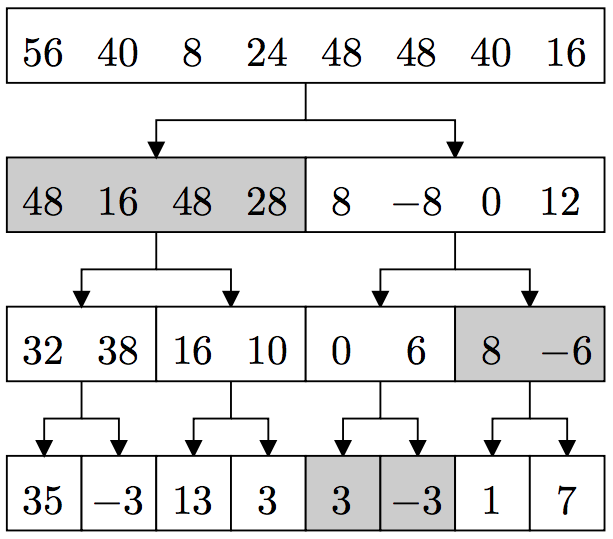
\includegraphics[width=0.8\textwidth]{fig/example1.png}
    \caption{An example of DWT on a signal with 8 elements.}
    \label{fig:example1}
\end{figure}



From the perspective of computational models in parallel computing, 
stencil




\section{Single Instruction Multiple Data}
\cite{lee1994parallel}

\bibliographystyle{plainyr} 
%\bibliographystyle{plain}
\bibliography{main}
\end{document}

